\documentclass[12pt]{article}
\usepackage{amsmath}
\usepackage{graphicx}
\usepackage{hyperref}
\usepackage{listings}
\usepackage{color}
\usepackage{pythonhighlight}

\title{Operating System Course Report - First Half of the Semester}
\author{B class}
\date{\today}

\begin{document}

\maketitle
\newpage

\tableofcontents
\newpage

\section{Introduction}
This report summarizes the topics covered during the first half of the Operating System course. It includes theoretical concepts, practical implementations, and assignments. The course focuses on the fundamentals of operating systems, including system architecture, process management, CPU scheduling, and deadlock handling.

\section{Course Overview}
\subsection{Objectives}
The main objectives of this course are:
\begin{itemize}
    \item To understand the basic components and architecture of a computer system.
    \item To learn process management, scheduling, and inter-process communication.
    \item To explore file systems, input/output management, and virtualization.
    \item To study the prevention and handling of deadlocks in operating systems.
\end{itemize}

\subsection{Course Structure}
The course is divided into two halves. This report focuses on the first half, which covers:
\begin{itemize}
    \item Basic Concepts and Components of Computer Systems
    \item System Performance and Metrics
    \item System Architecture of Computer Systems
    \item Process Description and Control
    \item Scheduling Algorithms
    \item Process Creation and Termination
    \item Introduction to Threads
    \item File Systems
    \item Input and Output Management
    \item Deadlock Introduction and Prevention
    \item User Interface Management
    \item Virtualization in Operating Systems
\end{itemize}

\section{Topics Covered}

\subsection{Basic Concepts and Components of Computer Systems}
This section explains the fundamental components that make up a computer system, including the CPU, memory, storage, and input/output devices.

\subsection{System Performance and Metrics}
This section introduces various system performance metrics used to measure the efficiency of a computer system, including throughput, response time, and utilization.

\subsection{System Architecture of Computer Systems}
Describes the architecture of modern computer systems, focusing on the interaction between hardware and the operating system.

\subsection{Process Description and Control}
Processes are a central concept in operating systems. This section covers:
\subsubsection{Definition of Process}
\subsubsection{Process states and state transitions}

\subsubsection{Process Control Block (PCB)}
Process Control Block (PCB) adalah struktur data yang digunakan oleh sistem operasi untuk menyimpan semua informasi yang diperlukan tentang proses. PCB sangat penting untuk mengelola dan mengontrol proses yang sedang berjalan. PCB berfungsi sebagai representasi dari proses dalam memori dan memfasilitasi manajemen dan penjadwalan proses yang efisien.

PCB terdiri dari beberapa elemen informasi yang berhubungan dengan proses, termasuk:
\begin{itemize}
\item \textbf{Process ID (PID)}: Setiap proses memiliki ID unik yang digunakan oleh sistem operasi untuk membedakan satu proses dari yang lain.
\item \textbf{Process State}: Menyimpan keadaan saat ini dari proses seperti New, Ready, Running, Waiting, atau Terminated.
\item \textbf{Program Counter}: Menyimpan alamat dari instruksi berikutnya yang akan dieksekusi oleh proses.
\item \textbf{CPU Registers}: Menyimpan nilai dari register CPU yang digunakan oleh proses, termasuk register umum dan register status.
\item \textbf{Memory Management Information}: Berisi informasi tentang manajemen memori untuk proses, termasuk base dan limit register atau informasi halaman.
\item \textbf{I/O Status Information}: Menyimpan informasi tentang perangkat I/O yang digunakan oleh proses, termasuk daftar perangkat I/O yang sedang digunakan dan statusnya.
\item \textbf{Scheduling Information}: Menyimpan informasi yang diperlukan untuk penjadwalan proses, seperti prioritas proses dan pointer ke antrean penjadwalan.
\end{itemize}

\subsubsection{Context Switching}
\begin{figure}[h]
\centering
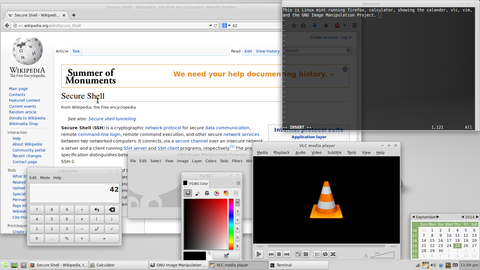
\includegraphics[width=0.6\textwidth]{asset/gambar_multitasking.png}
\caption{contoh proses multitasking}
\end{figure}

Context switching adalah proses di mana CPU beralih dari satu proses ke proses lain. Ini adalah mekanisme penting dalam sistem operasi multitasking yang memungkinkan beberapa proses untuk berbagi CPU.

Langkah-langkah dalam context switching meliputi:
\begin{itemize}
\item \textbf{Menyimpan Status Proses yang Berjalan}:
Sistem operasi menyimpan konteks proses yang sedang berjalan, termasuk isi register CPU (seperti accumulator, instruction pointer, flags), serta informasi lain seperti program counter dan status memori.
\item \textbf{Memilih Proses Baru}:
Sistem operasi memilih proses lain dari antrean ready untuk mulai dieksekusi. Proses ini dilakukan oleh penjadwal proses yang bertanggung jawab untuk menentukan proses mana yang harus diberi akses ke CPU.
\item \textbf{Memulihkan Status Proses yang Dipilih}:
Sistem operasi memuat kembali konteks dari proses yang telah dipilih untuk dieksekusi.
\item \textbf{Eksekusi Proses Baru}:
Setelah proses baru dipulihkan, CPU mulai mengeksekusi instruksi dari proses tersebut.
\end{itemize}

\subsubsection{Process Management By Operating Systems}
\subsection{Scheduling Algorithms}
This section covers:
\begin{itemize}
    \item First-Come, First-Served (FCFS)
    \item Shortest Job Next (SJN)
    \item Round Robin (RR)
\end{itemize}
It explains how these algorithms are used to allocate CPU time to processes.

\subsection{Process Creation and Termination}
Details how processes are created and terminated by the operating system, including:
\begin{itemize}
    \item Process spawning
    \item Process termination conditions
\end{itemize}

\subsection{Introduction to Threads}
This section introduces the concept of threads and their relation to processes, covering:
\begin{itemize}
    \item Single-threaded vs. multi-threaded processes
    \item Benefits of multithreading
\end{itemize}

\begin{figure}[h]
    \centering
    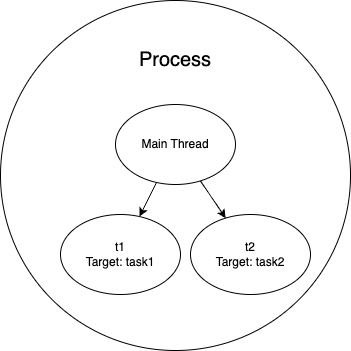
\includegraphics[width=0.5\textwidth]{asset/example.png}  % Sesuaikan nama file dan ukurannya
    \caption{Ini adalah gambar contoh dari multithreading.}
    \label{fig:contoh_gambar}
\end{figure}

Seperti yang terlihat pada Gambar \ref{fig:contoh_gambar}, inilah cara menambahkan gambar dengan keterangan.

\subsection{File Systems}
File systems provide a way for the operating system to store, retrieve, and manage data. This section explains:
\begin{itemize}
    \item File system structure
    \item File access methods
    \item Directory management
\end{itemize}

\subsection{Input and Output Management}
Input and output management is key for handling the interaction between the system and external devices. This section includes:
\begin{itemize}
    \item Device drivers
    \item I/O scheduling
\end{itemize}

\subsection{Deadlock Introduction and Prevention}
Explores the concept of deadlocks and methods for preventing them:
\begin{itemize}
    \item Deadlock conditions
    \item Deadlock prevention techniques
\end{itemize}

\subsection{User Interface Management}
This section discusses the role of the operating system in managing the user interface. Topics covered include:
\begin{itemize}
    \item Graphical User Interface (GUI)
    \item Command-Line Interface (CLI)
    \item Interaction between the user and the operating system
\end{itemize}

\subsection{Virtualization in Operating Systems}
Virtualization allows multiple operating systems to run concurrently on a single physical machine. This section explores:
\begin{itemize}
    \item Concept of virtualization
    \item Hypervisors and their types
    \item Benefits of virtualization in modern computing
\end{itemize}

\section{Assignments and Practical Work}
\subsection{Assignment 1: Process Scheduling}
Students were tasked with implementing various process scheduling algorithms (e.g., FCFS, SJN, and RR) and comparing their performance under different conditions.
\subsubsection{Group 1}
\begin{python}
    class Process:
    def __init__(self, pid, arrival_time, burst_time):
        self.pid = pid
        self.arrival_time = arrival_time
        self.burst_time = burst_time
        self.completion_time = 0
        self.turnaround_time = 0
        self.waiting_time = 0
\end{python}

\begin{table}[htbp] % Optional: For floating position
    \centering
    \begin{tabular}{|c|c|c|} % Defines number of columns and alignment (c = center, l = left, r = right). '|' creates vertical lines.
    \hline
    Header 1 & Header 2 & Header 3 \\ % Column headers
    \hline
    Row 1, Column 1 & Row 1, Column 2 & Row 1, Column 3 \\ % First row of data
    \hline
    Row 2, Column 1 & Row 2, Column 2 & Row 2, Column 3 \\ % Second row of data
    \hline
    \end{tabular}
    \caption{Your table caption} % Optional: For adding a caption
    \label{tab:your_label} % Optional: For cross-referencing the table
\end{table}

\subsection{Assignment 2: Deadlock Handling}
In this assignment, students were asked to simulate different deadlock scenarios and explore various prevention methods.

\subsection{Assignment 3: Multithreading and Amdahl's Law}
This assignment involved designing a multithreading scenario to solve a computationally intensive problem. Students then applied **Amdahl's Law** to calculate the theoretical speedup of the program as the number of threads increased.

\subsection{Assignment 4: Simple Command-Line Interface (CLI) for User Interface Management}
Students were tasked with creating a simple **CLI** for user interface management. The CLI should support basic commands such as file manipulation (creating, listing, and deleting files), process management, and system status reporting.

\subsection{Assignment 5: File System Access}
In this assignment, students implemented file system access routines, including:
\begin{itemize}
    \item File creation and deletion
    \item Reading from and writing to files
    \item Navigating directories and managing file permissions
\end{itemize}

\section{Conclusion}
The first half of the course introduced core operating system concepts, including process management, scheduling, multithreading, and file system access. These topics provided a foundation for more advanced topics to be covered in the second half of the course.

\begin{thebibliography}{}
    \bibitem{}
    Tutorialspoint. (n.d.). \textit{Operating system - Process control block}. Diakses pada 30 September 2024, dari \url{https://www.tutorialspoint.com/operating_system/os_process_control_block.htm}
    \bibitem{}
    Wikipedia contributors. (n.d.). Context switch. Dalam \textit{Wikipedia, The Free Encyclopedia}. Diakses pada 30 September 2024, dari \url{https://en.wikipedia.org/wiki/Context_switch} 
\end{thebibliography}

\end{document}